% Options for packages loaded elsewhere
\PassOptionsToPackage{unicode}{hyperref}
\PassOptionsToPackage{hyphens}{url}
%
\documentclass[
]{article}
\usepackage{amsmath,amssymb}
\usepackage{lmodern}
\usepackage{iftex}
\ifPDFTeX
  \usepackage[T1]{fontenc}
  \usepackage[utf8]{inputenc}
  \usepackage{textcomp} % provide euro and other symbols
\else % if luatex or xetex
  \usepackage{unicode-math}
  \defaultfontfeatures{Scale=MatchLowercase}
  \defaultfontfeatures[\rmfamily]{Ligatures=TeX,Scale=1}
\fi
% Use upquote if available, for straight quotes in verbatim environments
\IfFileExists{upquote.sty}{\usepackage{upquote}}{}
\IfFileExists{microtype.sty}{% use microtype if available
  \usepackage[]{microtype}
  \UseMicrotypeSet[protrusion]{basicmath} % disable protrusion for tt fonts
}{}
\makeatletter
\@ifundefined{KOMAClassName}{% if non-KOMA class
  \IfFileExists{parskip.sty}{%
    \usepackage{parskip}
  }{% else
    \setlength{\parindent}{0pt}
    \setlength{\parskip}{6pt plus 2pt minus 1pt}}
}{% if KOMA class
  \KOMAoptions{parskip=half}}
\makeatother
\usepackage{xcolor}
\usepackage[margin=1in]{geometry}
\usepackage{color}
\usepackage{fancyvrb}
\newcommand{\VerbBar}{|}
\newcommand{\VERB}{\Verb[commandchars=\\\{\}]}
\DefineVerbatimEnvironment{Highlighting}{Verbatim}{commandchars=\\\{\}}
% Add ',fontsize=\small' for more characters per line
\usepackage{framed}
\definecolor{shadecolor}{RGB}{248,248,248}
\newenvironment{Shaded}{\begin{snugshade}}{\end{snugshade}}
\newcommand{\AlertTok}[1]{\textcolor[rgb]{0.94,0.16,0.16}{#1}}
\newcommand{\AnnotationTok}[1]{\textcolor[rgb]{0.56,0.35,0.01}{\textbf{\textit{#1}}}}
\newcommand{\AttributeTok}[1]{\textcolor[rgb]{0.77,0.63,0.00}{#1}}
\newcommand{\BaseNTok}[1]{\textcolor[rgb]{0.00,0.00,0.81}{#1}}
\newcommand{\BuiltInTok}[1]{#1}
\newcommand{\CharTok}[1]{\textcolor[rgb]{0.31,0.60,0.02}{#1}}
\newcommand{\CommentTok}[1]{\textcolor[rgb]{0.56,0.35,0.01}{\textit{#1}}}
\newcommand{\CommentVarTok}[1]{\textcolor[rgb]{0.56,0.35,0.01}{\textbf{\textit{#1}}}}
\newcommand{\ConstantTok}[1]{\textcolor[rgb]{0.00,0.00,0.00}{#1}}
\newcommand{\ControlFlowTok}[1]{\textcolor[rgb]{0.13,0.29,0.53}{\textbf{#1}}}
\newcommand{\DataTypeTok}[1]{\textcolor[rgb]{0.13,0.29,0.53}{#1}}
\newcommand{\DecValTok}[1]{\textcolor[rgb]{0.00,0.00,0.81}{#1}}
\newcommand{\DocumentationTok}[1]{\textcolor[rgb]{0.56,0.35,0.01}{\textbf{\textit{#1}}}}
\newcommand{\ErrorTok}[1]{\textcolor[rgb]{0.64,0.00,0.00}{\textbf{#1}}}
\newcommand{\ExtensionTok}[1]{#1}
\newcommand{\FloatTok}[1]{\textcolor[rgb]{0.00,0.00,0.81}{#1}}
\newcommand{\FunctionTok}[1]{\textcolor[rgb]{0.00,0.00,0.00}{#1}}
\newcommand{\ImportTok}[1]{#1}
\newcommand{\InformationTok}[1]{\textcolor[rgb]{0.56,0.35,0.01}{\textbf{\textit{#1}}}}
\newcommand{\KeywordTok}[1]{\textcolor[rgb]{0.13,0.29,0.53}{\textbf{#1}}}
\newcommand{\NormalTok}[1]{#1}
\newcommand{\OperatorTok}[1]{\textcolor[rgb]{0.81,0.36,0.00}{\textbf{#1}}}
\newcommand{\OtherTok}[1]{\textcolor[rgb]{0.56,0.35,0.01}{#1}}
\newcommand{\PreprocessorTok}[1]{\textcolor[rgb]{0.56,0.35,0.01}{\textit{#1}}}
\newcommand{\RegionMarkerTok}[1]{#1}
\newcommand{\SpecialCharTok}[1]{\textcolor[rgb]{0.00,0.00,0.00}{#1}}
\newcommand{\SpecialStringTok}[1]{\textcolor[rgb]{0.31,0.60,0.02}{#1}}
\newcommand{\StringTok}[1]{\textcolor[rgb]{0.31,0.60,0.02}{#1}}
\newcommand{\VariableTok}[1]{\textcolor[rgb]{0.00,0.00,0.00}{#1}}
\newcommand{\VerbatimStringTok}[1]{\textcolor[rgb]{0.31,0.60,0.02}{#1}}
\newcommand{\WarningTok}[1]{\textcolor[rgb]{0.56,0.35,0.01}{\textbf{\textit{#1}}}}
\usepackage{graphicx}
\makeatletter
\def\maxwidth{\ifdim\Gin@nat@width>\linewidth\linewidth\else\Gin@nat@width\fi}
\def\maxheight{\ifdim\Gin@nat@height>\textheight\textheight\else\Gin@nat@height\fi}
\makeatother
% Scale images if necessary, so that they will not overflow the page
% margins by default, and it is still possible to overwrite the defaults
% using explicit options in \includegraphics[width, height, ...]{}
\setkeys{Gin}{width=\maxwidth,height=\maxheight,keepaspectratio}
% Set default figure placement to htbp
\makeatletter
\def\fps@figure{htbp}
\makeatother
\setlength{\emergencystretch}{3em} % prevent overfull lines
\providecommand{\tightlist}{%
  \setlength{\itemsep}{0pt}\setlength{\parskip}{0pt}}
\setcounter{secnumdepth}{-\maxdimen} % remove section numbering
\usepackage{amsmath,amssymb}
\usepackage[utf8]{inputenc}
\ifLuaTeX
  \usepackage{selnolig}  % disable illegal ligatures
\fi
\IfFileExists{bookmark.sty}{\usepackage{bookmark}}{\usepackage{hyperref}}
\IfFileExists{xurl.sty}{\usepackage{xurl}}{} % add URL line breaks if available
\urlstyle{same} % disable monospaced font for URLs
\hypersetup{
  pdftitle={Exercice n°2},
  pdfauthor={Grégoire de Lambertye},
  hidelinks,
  pdfcreator={LaTeX via pandoc}}

\title{Exercice n°2}
\usepackage{etoolbox}
\makeatletter
\providecommand{\subtitle}[1]{% add subtitle to \maketitle
  \apptocmd{\@title}{\par {\large #1 \par}}{}{}
}
\makeatother
\subtitle{Random Number Generation through CDF and acceptance-rejection
sampling}
\author{Grégoire de Lambertye}
\date{2022-10-10}

\begin{document}
\maketitle

\hypertarget{pseudo-random-number-generation-with-linear-congruential-random-number-generation-algorithm}{%
\section{Pseudo-random number generation with Linear Congruential Random
Number Generation
Algorithm}\label{pseudo-random-number-generation-with-linear-congruential-random-number-generation-algorithm}}

Pseudo-random number generators (PRNG) are algorithms used in computer
science to simulate random number generation. They are called pseudo
because they use recursive process to generate numbers and they are
initialized with a seed. They are by this way reproducible and
deterministic but they look random.

The main idea of the linear congruential random number generator is to
define a sequence based on the linear formula
\({x_n+1} = (a · x_n + c) (m)\)

Here is a linear congruential number generator :

That we can observe here

\begin{Shaded}
\begin{Highlighting}[]
\FunctionTok{plot}\NormalTok{(}\FunctionTok{congruential\_gen}\NormalTok{(}\DecValTok{100}\NormalTok{,}\DecValTok{178}\NormalTok{,}\DecValTok{3}\NormalTok{,}\DecValTok{44}\NormalTok{,}\DecValTok{72}\NormalTok{), }\AttributeTok{main=}\StringTok{"Random number generator"}\NormalTok{, }\AttributeTok{ylab=}\StringTok{"Random values"}\NormalTok{)}
\end{Highlighting}
\end{Shaded}

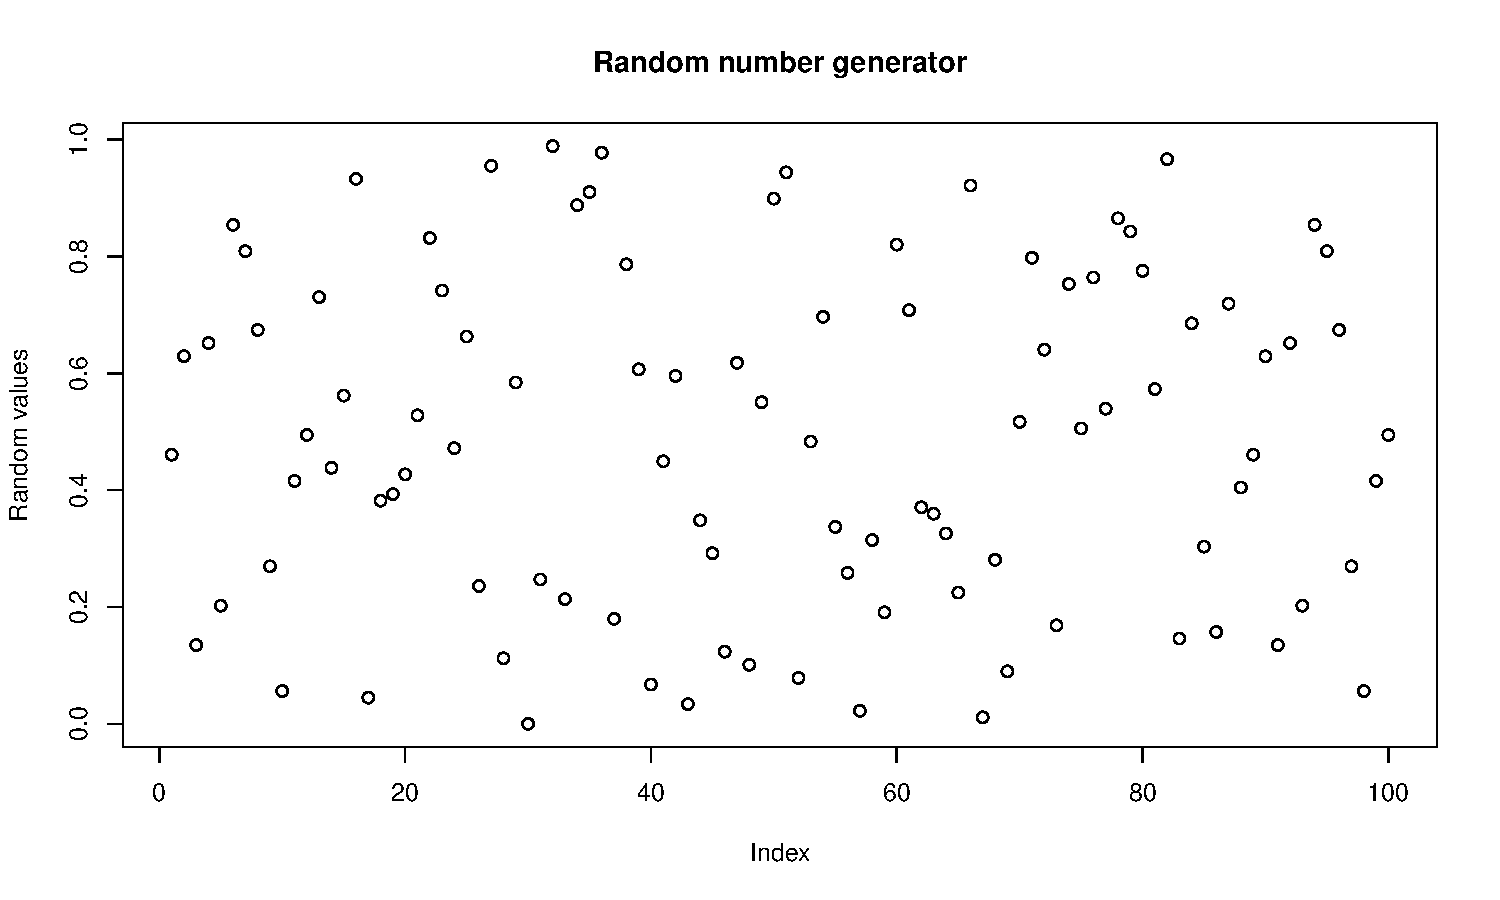
\includegraphics{Exercicen2_files/figure-latex/unnamed-chunk-2-1.pdf}
The modulus number m as a huge influence on the sequence and act as a
``maximal number generated'' befor the mapping between 0 and 1. It also
a major parameter for the sequence length. With a small m, it's easy to
recognize the sequence quickly:

\begin{Shaded}
\begin{Highlighting}[]
\FunctionTok{plot}\NormalTok{(}\FunctionTok{congruential\_gen}\NormalTok{(}\DecValTok{15}\NormalTok{,}\DecValTok{5}\NormalTok{,}\DecValTok{7}\NormalTok{,}\DecValTok{2}\NormalTok{,}\DecValTok{0}\NormalTok{), }\AttributeTok{main=}\StringTok{"Random number generator m=5"}\NormalTok{, }\AttributeTok{ylab=}\StringTok{"Random numbers"}\NormalTok{)}
\FunctionTok{plot}\NormalTok{(}\FunctionTok{congruential\_gen}\NormalTok{(}\DecValTok{15}\NormalTok{,}\DecValTok{20}\NormalTok{,}\DecValTok{7}\NormalTok{,}\DecValTok{2}\NormalTok{,}\DecValTok{4}\NormalTok{), }\AttributeTok{main=}\StringTok{"Random number generator m=20"}\NormalTok{, }\AttributeTok{ylab=}\StringTok{"Random numbers"}\NormalTok{)}
\FunctionTok{plot}\NormalTok{(}\FunctionTok{congruential\_gen}\NormalTok{(}\DecValTok{15}\NormalTok{,}\DecValTok{150}\NormalTok{,}\DecValTok{7}\NormalTok{,}\DecValTok{2}\NormalTok{,}\DecValTok{4}\NormalTok{), }\AttributeTok{main=}\StringTok{"Random number generator m=150"}\NormalTok{, }\AttributeTok{ylab=}\StringTok{"Random numbers"}\NormalTok{)}
\end{Highlighting}
\end{Shaded}

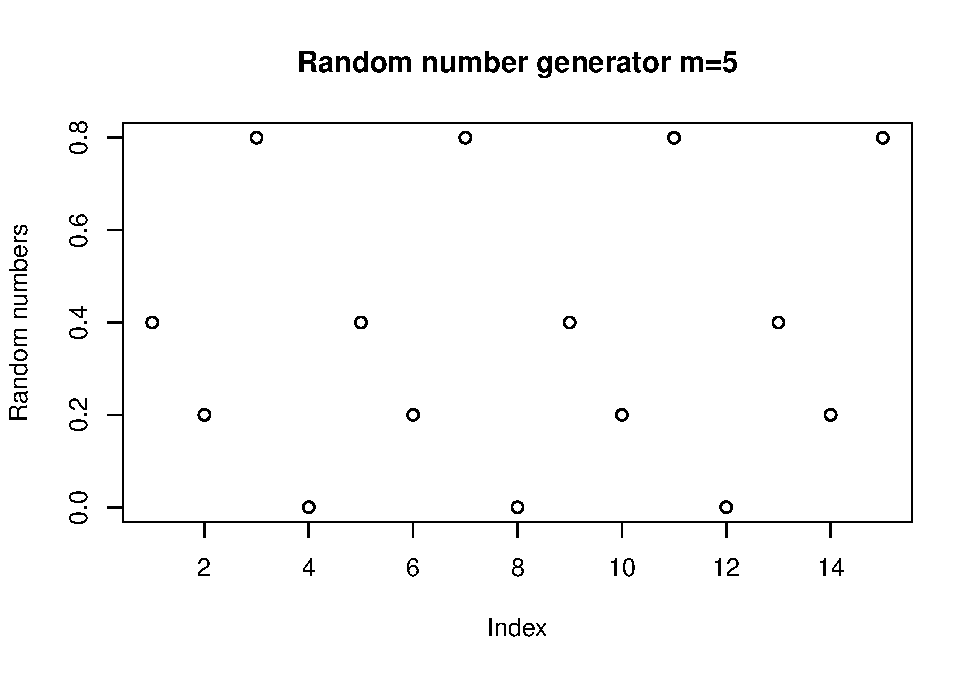
\includegraphics[width=0.5\linewidth]{Exercicen2_files/figure-latex/unnamed-chunk-3-1}
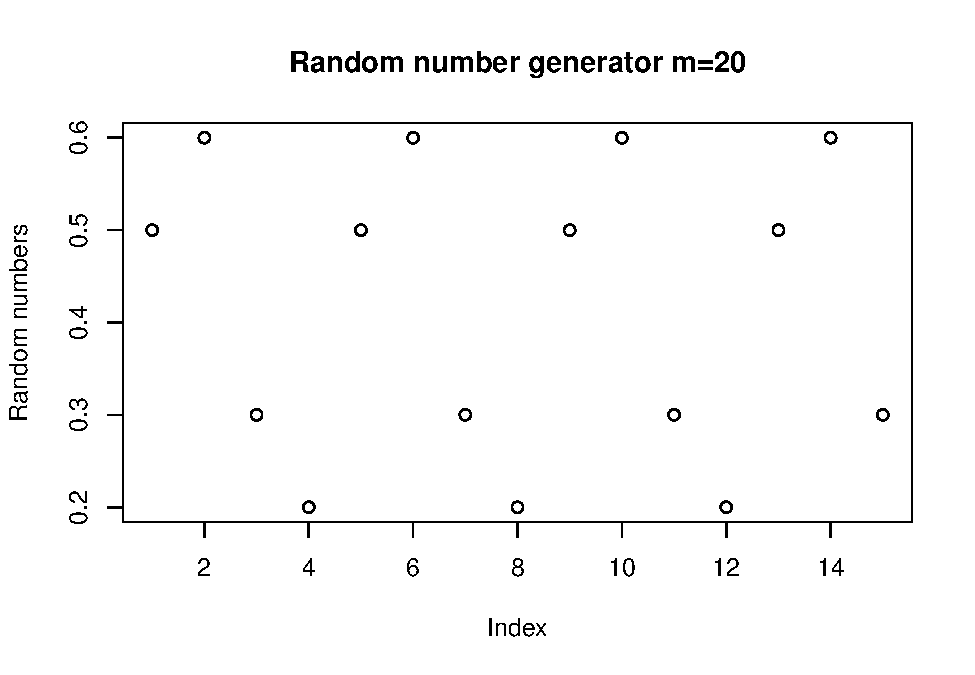
\includegraphics[width=0.5\linewidth]{Exercicen2_files/figure-latex/unnamed-chunk-3-2}
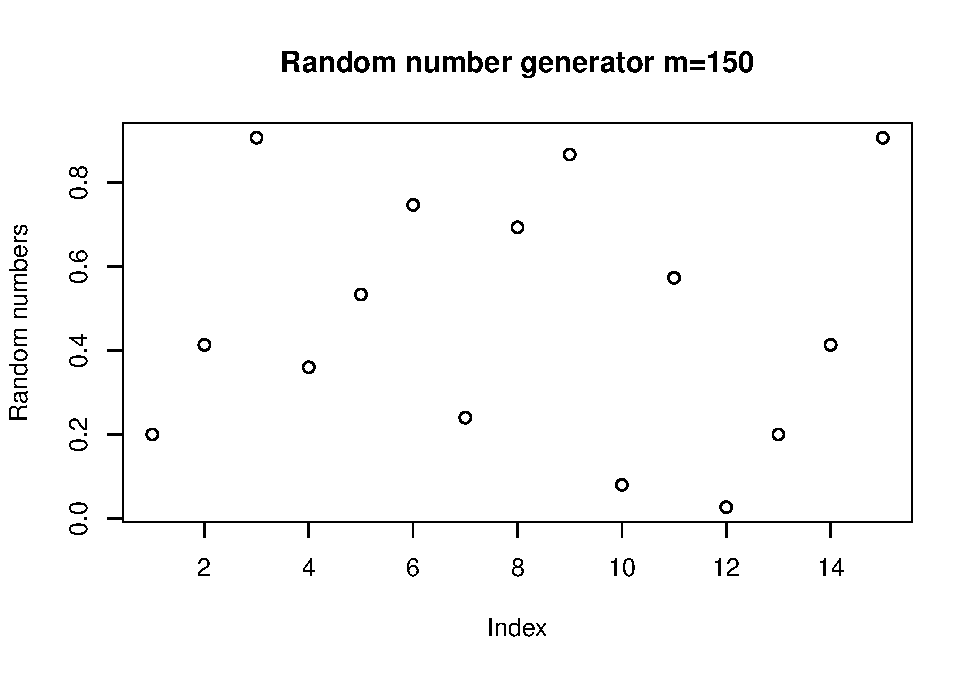
\includegraphics[width=0.5\linewidth]{Exercicen2_files/figure-latex/unnamed-chunk-3-3}
It seems pretty easy to understand the sequence of the 2 firsts plot.
For the m=150 sample we would need more data to be able to recognize the
sequence.

\hypertarget{exponential-distribution}{%
\section{Exponential distribution}\label{exponential-distribution}}

The exponetial function is obtain with this equation :
\(F(x) = 1-exp(-λx), λ>0\)

\begin{Shaded}
\begin{Highlighting}[]
\NormalTok{expf }\OtherTok{\textless{}{-}} \ControlFlowTok{function}\NormalTok{(x, lambda)\{}
  \FunctionTok{return}\NormalTok{(}\DecValTok{1}\SpecialCharTok{{-}}\FunctionTok{exp}\NormalTok{(}\SpecialCharTok{{-}}\NormalTok{lambda}\SpecialCharTok{*}\NormalTok{x))}
\NormalTok{\}}
\end{Highlighting}
\end{Shaded}

Assume you can generate easily uniform random variables. How can you
obtain then a random sample from the exponential distribution? use .
Compute the quantile function F−1x. =\textgreater{} F−1 X (u) = inf\{x :
FX (x) ≥ u\} 2. Generate a u ∼ unif {[}0, 1{]}. 3. Make the
transformation x = F −1 X (u)

\begin{Shaded}
\begin{Highlighting}[]
\NormalTok{x }\OtherTok{=} \FunctionTok{seq}\NormalTok{(}\AttributeTok{from=}\SpecialCharTok{{-}}\DecValTok{2}\NormalTok{, }\AttributeTok{to=}\DecValTok{2}\NormalTok{, }\AttributeTok{length.out=}\DecValTok{200}\NormalTok{)}
\NormalTok{res }\OtherTok{\textless{}{-}} \FunctionTok{c}\NormalTok{()}

\ControlFlowTok{for}\NormalTok{(i }\ControlFlowTok{in}\NormalTok{ x)\{}
\NormalTok{  res }\OtherTok{\textless{}{-}} \FunctionTok{append}\NormalTok{(res, }\FunctionTok{expf}\NormalTok{(i,}\DecValTok{3}\NormalTok{))}
\NormalTok{\}}

\FunctionTok{plot}\NormalTok{(res)}
\end{Highlighting}
\end{Shaded}

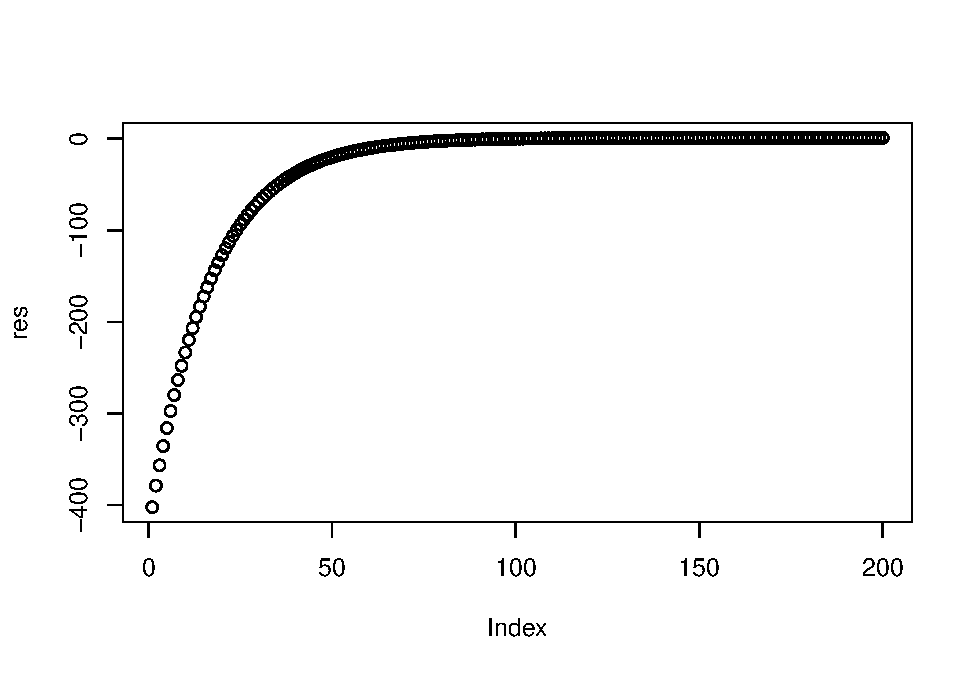
\includegraphics{Exercicen2_files/figure-latex/unnamed-chunk-6-1.pdf}

\end{document}
